\documentclass{article}
\usepackage{tikz}
\usepackage{geometry}
\usepackage{fancyhdr}
\usepackage{enumitem}
\usepackage{amsmath}
\usepackage{hyperref}
\usetikzlibrary{arrows}

\geometry{letterpaper, left=1cm, right=1cm, top=2cm, bottom=2cm}

\pagestyle{fancy}
\fancyhf{}
\renewcommand{\headrulewidth}{0pt}
\fancyfoot[LE,RO]{\thepage}
\fancyfoot[RE,LO]{\copyright\hspace{0.25em}codeabode 2025. \href{https://codeabode.co}{\underline{codeabode.co}}}

\title{\vspace{-3em}Collisions Worksheet\vspace{-2em}}

\begin{document}

\maketitle


\begin{center}
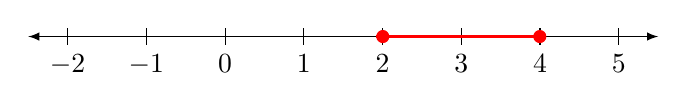
\begin{tikzpicture}
    \draw[latex-latex] (-2.5,0) -- (5.5,0) ; %edit here for the axis
        \foreach \x in  {-2,-1,0,1,2,3,4,5} % edit here for the vertical lines
        \draw[shift={(\x,0)},color=black] (0pt,3pt) -- (0pt,-3pt);
        \foreach \x in {-2,-1,0,1,2,3,4,5} % edit here for the numbers
        \draw[shift={(\x,0)},color=black] (0pt,0pt) -- (0pt,-3pt) node[below] 
        {$\x$};
        \draw[*-*,color=red] (1.92,0) -- (4.08,0);
        \draw[very thick,color=red] (1.92,0) -- (3.92,0);
    \end{tikzpicture}
\end{center}

\begin{enumerate}
   
    \item What is the $x$ value of the red block? Hint: always top-left
    
    \rule{3cm}{0.4pt}

    \item How wide is the red block?

    \rule{3cm}{0.4pt}


% here is a thing with width 5, make it overlap, they draw evt
% one xy axis overlap problem
    
\end{enumerate}


\begin{center}
    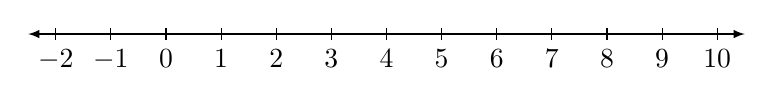
\begin{tikzpicture}[scale=0.7]
    \draw[latex-latex] (-2.5,0) -- (10.5,0) ; %edit here for the axis
        \foreach \x in  {-2,-1,0,1,2,3,4,5,6,7,8,9,10} % edit here for the vertical lines
        \draw[shift={(\x,0)},color=black] (0pt,3pt) -- (0pt,-3pt);
        \foreach \x in {-2,-1,0,1,2,3,4,5,6,7,8,9,10} % edit here for the numbers
        \draw[shift={(\x,0)},color=black] (0pt,0pt) -- (0pt,-3pt) node[below] 
        {$\x$};
    \end{tikzpicture}
\end{center}

\begin{enumerate}
    \item Draw a block at $x=-1$ that is 5 units wide.
    \item Draw a block at $x=3$ that is 2 units wide.
    \item Do they overlap?

    \rule{3cm}{0.4pt}
\end{enumerate}

\begin{center}
    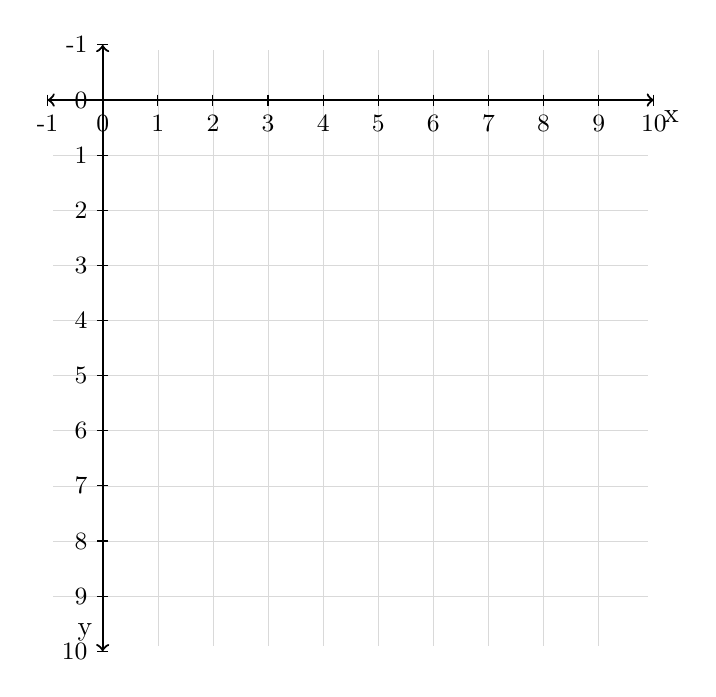
\begin{tikzpicture}[scale=0.7]
        \draw[gray!30, very thin, step=1] (-0.9,0.9) grid (9.9,-9.9);
        \draw[thick, <->] (-1,0) -- (10,0) node[below right] {x};
        \draw[thick, <->] (0,1) -- (0,-10) node[above left] {y};
        \foreach \x in {-1,0,...,10} {
            \draw (\x,0.1) -- (\x,-0.1) node[below] {\small\x};
        }
        \foreach \y in {1,0,...,-10} {
            \draw (0.1,\y) -- (-0.1,\y) node[left] {\small\the\numexpr-\y\relax};
        }
    \end{tikzpicture}
\end{center}

\begin{enumerate}
    \item Draw a rectangle at $x=3$, $y=2$, width=3, height=2.
    \item Draw a rect $(6,3,2,1)$, where each number is $(x,y,\text{width},\text{height})$
    \item Do they overlap?

    \rule{3cm}{0.4pt}
\end{enumerate}


\begin{center}
    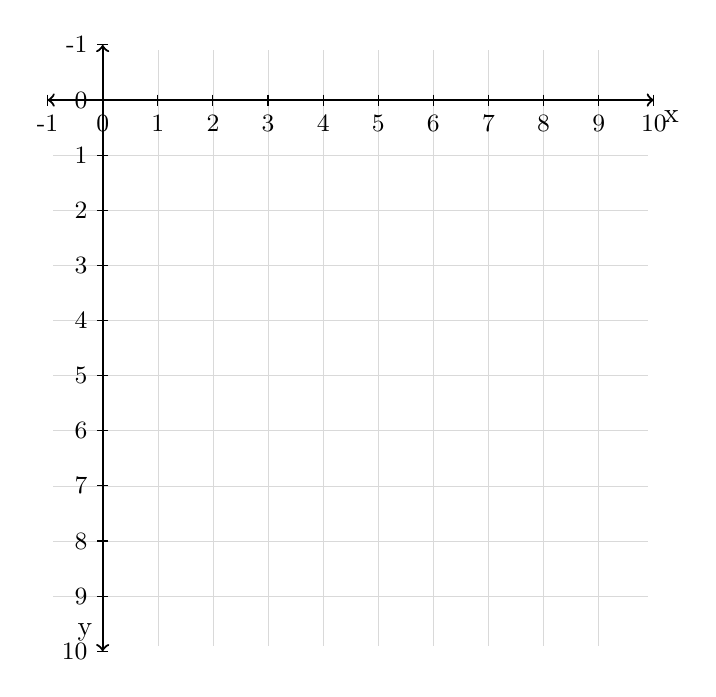
\begin{tikzpicture}[scale=0.7]
        \draw[gray!30, very thin, step=1] (-0.9,0.9) grid (9.9,-9.9);
        \draw[thick, <->] (-1,0) -- (10,0) node[below right] {x};
        \draw[thick, <->] (0,1) -- (0,-10) node[above left] {y};
        \foreach \x in {-1,0,...,10} {
            \draw (\x,0.1) -- (\x,-0.1) node[below] {\small\x};
        }
        \foreach \y in {1,0,...,-10} {
            \draw (0.1,\y) -- (-0.1,\y) node[left] {\small\the\numexpr-\y\relax};
        }
    \end{tikzpicture}
\end{center}

\begin{enumerate}
    \item Draw a rect at (1,1,6,6)
    \item Draw a rect at (4,2,1,1)
    \item Do they overlap?

    \rule{3cm}{0.4pt}
\end{enumerate}

\end{document}
